\documentclass{article}
\input{../../preamble.tex}
\usepackage[letterpaper, portrait, margin=1in]{geometry}
\usepackage{longtable}

\graphicspath{./figures}

\pagestyle{fancy}
\fancyhf{}
\lhead{Sidharth Baskaran}
\chead{Project Euler 54}
\rhead{01/13/2022}

\lstset{
	basicstyle=\ttfamily\scriptsize,
	frame=single,
	breaklines=true,
  numbers=left
}

\begin{document}
    
\section{Problem Statement}

In the card game poker, a hand consists of five cards and are ranked,
from lowest to highest, in the following way:

\begin{itemize}
\item
  \textbf{High Card}: Highest value card.
\item
  \textbf{One Pair}: Two cards of the same value.
\item
  \textbf{Two Pairs}: Two different pairs.
\item
  \textbf{Three of a Kind}: Three cards of the same value.
\item
  \textbf{Straight}: All cards are consecutive values.
\item
  \textbf{Flush}: All cards of the same suit.
\item
  \textbf{Full House}: Three of a kind and a pair.
\item
  \textbf{Four of a Kind}: Four cards of the same value.
\item
  \textbf{Straight Flush}: All cards are consecutive values of same
  suit.
\item
  \textbf{Royal Flush}: Ten, Jack, Queen, King, Ace, in same suit.
\end{itemize}

The cards are valued in the order:\\
2, 3, 4, 5, 6, 7, 8, 9, 10, Jack, Queen, King, Ace.

If two players have the same ranked hands then the rank made up of the
highest value wins; for example, a pair of eights beats a pair of fives
(see example 1 below). But if two ranks tie, for example, both players
have a pair of queens, then highest cards in each hand are compared (see
example 4 below); if the highest cards tie then the next highest cards
are compared, and so on.

Consider the following five hands dealt to two players:

\begin{figure}[H]
  \centering
  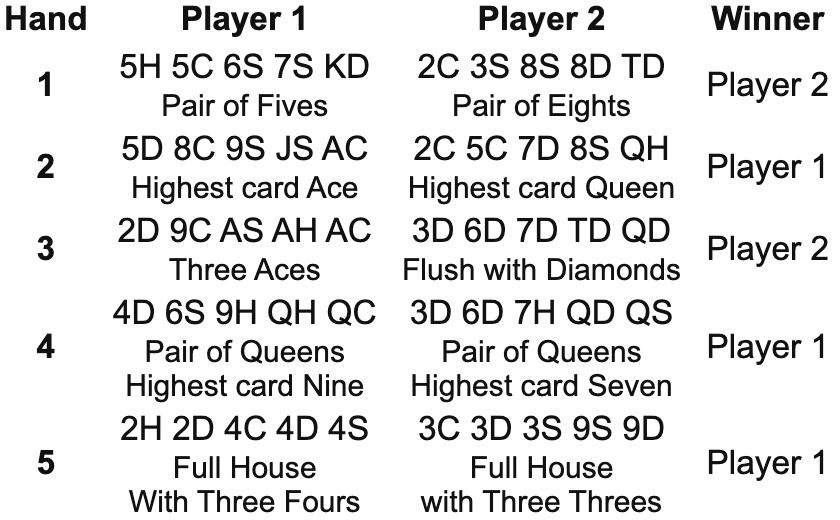
\includegraphics[scale=0.75]{../figures/poker.png}
  \caption{Example}
\end{figure}

The file, \href{project/resources/p054_poker.txt}{poker.txt}, contains
one-thousand random hands dealt to two players. Each line of the file
contains ten cards (separated by a single space): the first five are
Player 1's cards and the last five are Player 2's cards. You can assume
that all hands are valid (no invalid characters or repeated cards), each
player's hand is in no specific order, and in each hand there is a clear
winner.

\newpage

\section{Code}

\lstinputlisting[language=Python]{../code/54.py}

\section{Explanation}

This problem requires a brute-force approach to evaluate each game of poker presented in the file.
We are given the priorities of each card and the possible ranks. The code begins by initializing dictionaries called \verb|VALUES| and \verb|RANKS|
in order to assign an integer priority value to each rank and card value.

The \verb|score_hand| method takes in a hand of 5 cards determines its rank score by iterating through the possible
ranks, defined by succinct anonymous functions. The highest rank score is recorded and returned, along with other useful data: all rank scores for the hand, the card values, and the card frequency.

To solve the problem, we iterate through each of the thousand poker games given and compare the scores of the players, incrementing Player 1's count if there is no tie.
If there is a tie, we either consider the case of a tie where pairs of cards exist, or a tie without pairs of cards.
The rules of the game dictate that if a tie occurs where both players have the same ``paired'' rank (one pair, two pairs, three of a kind, full house, four of a kind),
the player with pairs of the highest value card takes priority. So the code takes the scores from each player pertaining to these 5 ``paired'' ranks, determines if there is a tie, and
removes all single occurences of cards from the hand (thus resulting in only pairs remaining). Then, we compare the maximum value from each player's pairs and increment the count if Player 1 wins.
If there is a simple tie, we check which player has the highest value card and increment Player 1's count if they do.

\end{document}